
\section{State Machine included mode}
\begin{wrapfigure}{r}{0.5\textwidth}
  \vspace{-30pt}
  \begin{center}
    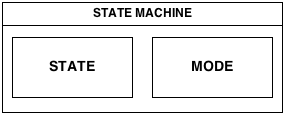
\includegraphics[width=0.48\textwidth]{pictures/StateMachine_mode.png}
  \end{center}
  \vspace{-20pt}
  \caption{StateMachine overview}
  \vspace{-10pt}
\end{wrapfigure}
The State Machine is now renewed whit the new mode part. First the State Machine was controlled by its state. Now the State Machine can be controlled by its state and its mode.

\subsection{Mode change}
Currently there is no transition between a mode change. Also it is possible to change every modes independent of its current mode. Perhaps this should implemented in the future to control the mode changes, but now it isn't necessary.

\subsection{State Machine addition}
The State Machine add functionality to influence the State Machine. This should be needed by modes. Each mode is designed by possible states and possible transitions.
\paragraph{Possible (transition)states}When the State Machine is in an non possible state, it abort. The abort of a transition state is it's contrary. The stop and shutdown transitions hasn't abort transitions. The abort of a state is it's lower transition state, such as: Normal=Stop and Standby=Shutdown. The Safe sate hasn't a abort.
\paragraph{Possible transitions}The State Machine change to an transition state only when it is in the possible transitions. If it isn't it is also not possible to change the state by this transition.

\subsection{Modes}
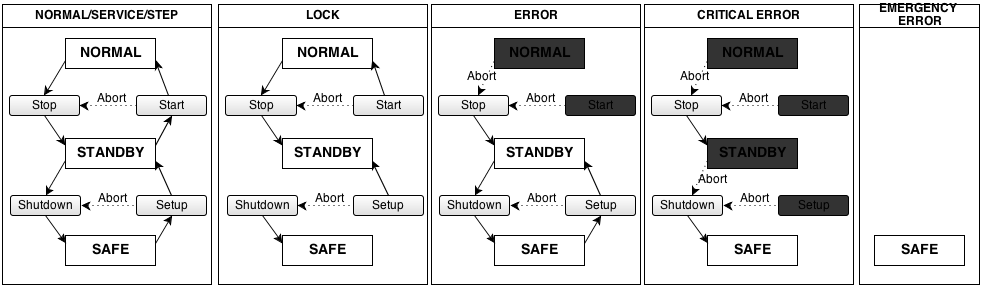
\includegraphics[width=1\textwidth]{pictures/modes.png}\\
The Equiplet used different standard modes which influence the State Machine. Each mode discribe the possible states and transitions. All states and transitions which are not in the possibles are non possible. 

\subsubsection{Normal}This mode will mean that the State Machine runs in original mode. There are no particularities in this mode.\\\\
\textbf{Possible (transitions)states:}Normal, Standby, Safe, Setup, Shutdown, Start, Stop\\
\textbf{Possible transitions:}Setup, Shutdown, Start, Stop

\subsubsection{Service}This mode will be used to have more control of the machine. It can be used to (re-)configurate the machine or to get debug information. In this mode the State Machine is allowed to executed as in the normal mode.\\\\
\textbf{Possible (transitions)states:}Normal, Standby, Safe, Setup, Shutdown, Start, Stop\\
\textbf{Possible transitions:}Setup, Shutdown, Start, Stop

\subsubsection{Step}This mode will means that Step control is enabled. The State Machine runs it's task by once and continue when a user set the next step.\\\\
\textbf{Possible (transitions)states:}Normal, Standby, Safe, Setup, Shutdown, Start, Stop\\
\textbf{Possible transitions:}Setup, Shutdown, Start, Stop

\subsubsection{Error}This mode is used when an error is on the machine, but it isn't a dangerous error for the machine. When the module in Normal it should to stop and it task and it isn't allowed to start a new task when in Standby.\\\\
\textbf{Possible (transitions)states:}Standby, Safe, Setup, Shutdown, Stop\\
\textbf{Possible transitions:}Setup, Shutdown, Stop

\subsubsection{Critical Error}This mode is used when a dangerous error is detected on the machine. Only the Safe state is possible in this state and when the State Machine isn't safe, it should force to Stop if necessary and Shutdown.\\\\
\textbf{Possible (transitions)states:}Safe, Shutdown, Stop\\
\textbf{Possible transitions:}Shutdown, Stop

\subsubsection{Emergency Stop}This mode should used when the emergency stop is pressed. In this mode the State Machine is set as safe, because an emergency stop isn't a software stop but a hardware stop.\\\\
\textbf{Possible (transitions)states:}Safe\\
\textbf{Possible transitions:}-

\subsubsection{Lock}This mode is used to lock a state in the State Machine. This is simply realized to remote the transitions, but only the the Stop transition has remained. When it has finish its task it isn't possible to stay in normal, because the normal state will means that the machine is running. On this reason the stop transition is possible in this mode. When the machine is in a transition state it should finish it transition\\\\
\textbf{Possible (transitions)states:}Normal, Standby, Safe, Setup, Shutdown, Start, Stop\\
\textbf{Possible transitions:} Shutdown, Stop

\section{Module}
The module create a Module StateMachine called as MOST(MOdule STate machine). This State Machine extends from the designed State Machine, but implement the State Machine with predefined modes. When a module extends the Module State Machine it must indicate if it is an actor or not. This is used to set the module in error, which will be done by the Module State Machine. An actor module set the State Machine in the 'critical error mode' and a non actor module set it in the 'error mode'. 

\subsection{MOST modes}
\paragraph{Normal}The normal State Machine mode.
\paragraph{Service}When the module in Service, it enable debug information and it allowed service methods to calibrate etc.
\paragraph{Error}This mode is used when an non actor module in error.
\paragraph{Critical error}This mode is used when an actor module sets an error. The State Machine will go to the safe.
\paragraph{Emergency error}This mode is used when the emergency button is pressed

\section{Equiplet}
\subsection{State Machine}
The Equiplet use also a State Machine to control its modules. This State Machine is called EST(Equiplet STate machine). The EST should be implemented in the ROS node.

\subsubsection{States}
\paragraph{Safe}The Equiplet is safe when all modules are also safe.
\paragraph{Standby}The standby state can be used when the modules of the Equiplet in standby state. Just as the module standby state indicate this a ready for run. This state is imported for the Equiplet because when the Equiplet isn’t ready to run, it isn’t possible to perform scheduled tasks directly. This is designed by the requirement of Erik Puik that an Equiplet only is ready to run when all modules are ready to run. When an module isn't ready to run, the Equiplet should now allowed to run.
\paragraph{Normal}This state is used when the Equiplet is executing an service step, i.e. the modules of the Equiplet are running the Equiplet steps. 

\subsubsection{Transitions}
\paragraph{Setup}Send to all modules of the Equiplet a change state to standby command. This transition is finished when all modules are standby.
\paragraph{Shutdown}Send to all modules of the Equiplet a change state to safe. This transition is finished when all modules are safe.
\paragraph{Start}It is starting a new service step and send the first Equiplet step to the module. When the module is normal, this transition finished.
\paragraph{Stop}It is stopping the service step. When all modules are standby the Equiplet change also to standby.

\subsubsection{Modes}
\paragraph{Normal}This mode is running when also all modules are normal
\paragraph{Service}When this mode is activated it set all modules in service.
\paragraph{Lock}This mode is to lock the Equiplet.
\paragraph{Step}This mode execute an Equiplet step by once. It send a new Equiplet step to a module when the EquipetStateMachine receive an next step command.
\paragraph{Emergency error}This mode is used when the emergency button is pressed
\paragraph{Error}The Equiplet activate this mode when a module is in error
\paragraph{Critical Error}The Equiplet activate this mode when a module is in critical error.

\subsection{State Blackboard}
To provide Equiplet agents from inform of the EST and MOST a blackboard should be used called the 'StateBlackboard'. This blackboard should be also used to allow the agent to change the state. The StateBlackboard provide the fallowing collections:
\paragraph{EquipletState}This collections contain the Equiplet states. It provides the 'safety state', the operational state and the Equiplet state. The safety- and the operational state provide only a state. The Equiplet state provide a Equiplet id, state and mode. 
\paragraph{EquipletCommands}By this blackboard the Equiplet state can be changed.
\paragraph{ModuleStates}This collection contains all module states. A module state contain of a: module id, module state and the module mode.

\subsection{Overview}
Now the Equiplet contains the fallowing states:
\begin{itemize}
\item Safety state which is the highest state of all modules
\item Operational state which is the lowest state required modules of a service step.
\item It's own Equiplet State provides from the Equiplet State Machine
\end{itemize}

\section{SCADA}
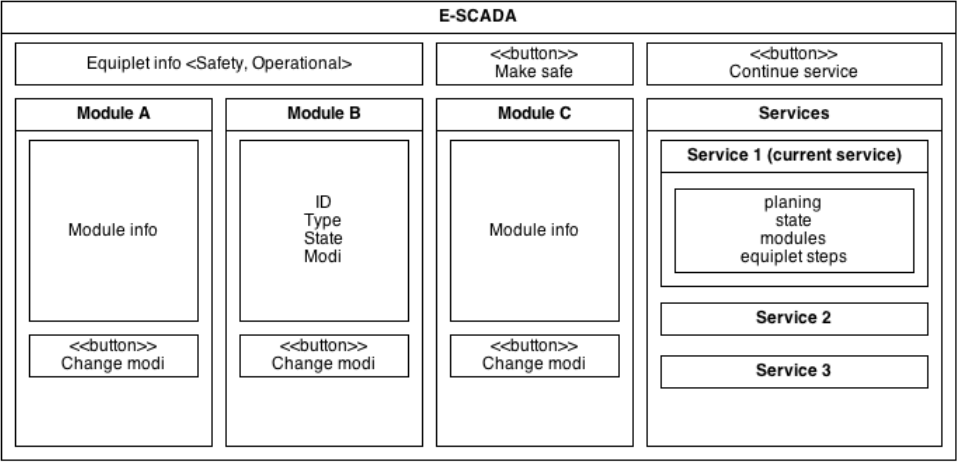
\includegraphics[width=1\textwidth]{pictures/SCADA.png}
The E-SCADA runs on the Equiplet PC and is a visual representation of everything happening in the Equiplet. 

\subsubsection{Equiplet information}
\begin{itemize}
\item Name/ID
\item Safety state
\item Operational state
\item Equiplet state
\end{itemize}
\subsubsection{Equiplet control}
\begin{itemize}
\item Make the Equiplet safe
\item Lock module
\item Continue step (step modi)
\end{itemize}
\subsubsection{Module information}
\begin{itemize}
\item Name/ID
\item Type
\item State
\item Modi
\end{itemize}
\subsubsection{Module control}
\begin{itemize}
\item Change module modi
\item Service information
\item Available services
\end{itemize}
\subsubsection{Scheduled services}
\begin{itemize}
\item Needed modules
\item Equiplet steps
\item Progress
\item Service state
\end{itemize}